%
%  nietzsche.one
%
%  Created by Mark Eli Kalderon on 2007-12-20.
%  Copyright (c) 2007 Mark Eli Kalderon. All rights reserved.
%
%  Beamer

% Definitions and macros
\newcommand{\change}{\textcolor{blue}{\textbf{CHANGE SLIDE}}}
\newcommand\myauthor{Mark Eli Kalderon} 
\newcommand\mytitle{Introduction to Moral Philosophy}
\newcommand\mysubtitle{Nietzsche}
\newcommand\myinstitution{University College London}
\newcommand\myurl{http://markelikalderon.com/teaching}

% Packages specific to lecture notes
\mode<article>{
    \usepackage{palatino}
    \setjobnamebeamerversion{nietzsche.one.beamer}
}

% Packages specific to beamer presentation
\mode<presentation>{
    \usetheme{Darmstadt}
    \setbeamercovered{transparent}
    \pgfdeclareimage[height=0.5cm]{university-logo}{../../graphics/logo_sml_blk}
    \logo{\pgfuseimage{university-logo}}
}

% Packages common to lecture notes and beamer presentation
\usepackage{pgf}
\usepackage{tikz}
\usepackage{hyperref}

\title{\mytitle}
\subtitle{\mysubtitle} % (optional)

\author{\myauthor\\
\url{\myurl}}
\institute{\myinstitution}

% \date[Short Occasion] % (optional)
% {Date / Occasion}

\begin{document}

\frame{\maketitle}

\section{The Problem of Style}\label{sec:the_problem_of_style} % (fold)

\change\ One of the features of Nietzsche's work that attracts some readers and repels others is Nietzsche's style. In one sense it is wrong to speak of Nietzsche's style because over the course of his literary output he used a vast variety of different styles. What is remarkable, however, is that one can always clearly discern Nietzsche's distinctive voice in whatever he writes no matter the specific style he happens to deploy. Nietzsche is perhaps the most literary of philosophers and it is worth commenting on his style because many of his philosophical doctrines are encoded in the literary character of his text. Indeed the argument of the \emph{Genealogy} ultimately depends on features of its literary style. This is an important issue that we will return to. But for now, let me underscore a couple of important points. It is a commonplace observation that an author writes so as to be understood. But Nietzsche also observes that just as importantly that there is a sense in which an author writes so as to \emph{not} be understood. Furthermore, this willfull fostering of misunderstanding is one of the important functions of literary style. Nietzsche discusses this ``antimony of style'' in the following passage from the \emph{Gay Science}:
\begin{quote}
    \emph{On the question of being understandable.}---One does not only wish to be understood when one writes; one wishes just as surely to be misunderstood. It is not by any means necessarily an objection to a book when anyone finds it impossible to understand: perhaps that was part of the author's intention---he did not want to be understood just by ``anybody''. All the nobler spirits and tastes select their audience when they wish to communicate; and choosing that, one at the same times erects barriers against the ``others''. All the most subtle laws of style have their origin at this point: they at the same time keep away, create a distance, forbid ``entrance'', understanding as said above---while they open the ears of those whose ears are related to ours.
\end{quote}
Style thus has a radically inegalitarian function. Literary style enforces the distinction between those capable of hearing Nietzsche's message and those who are incapable. Nietzsche does not write so as to be understood just by anyone---his text requires that his reader have certain literary and philosophical skills and indeed the accompanying virtues required to have these skills.

Just by way of preview, let me mention just one connection between Nietzsche's philosophical doctrine's and his literary style. One of the lesson's of the first essay of the \emph{Genealogy} is that novel values arise from a pre-established hierarchy or rank ordering. The sense of power accompanying such a rank order gives rise to values. Nietzsche describes this sense of power involved in the enforcing of a hierarchy ``the pathos of distance''. One of Nietzsche's fundamental ethical doctrine's is that moral values are only established given the prior establishment of some kind of hierarchy. Notice that there is a connection between what I described as the antimony of style and the pathos of distance. The antimony of style is just the observation that authors write not only to be understood but also to be misunderstood. That is to say, one of the functions of style is to insure that the text is only understood by his intended audience. Given this discriminatory function of style, the text itself creates a hierarchy or rank ordering which is a prerequisite for the creation of novel values. This observation is crucial in evaluating Nietzsche's overall argument of the \emph{Genealogy}.

Nietzsche makes a couple of remarks in the preface of the \emph{Genealogy} that bears on the question of its being understandable. In particular, he mentions two prerequisites for a proper understanding of the book. 

First, he presupposes an understanding of his previous works, themselves no easy matter to decipher. Do not put off by this. Hopefully my remarks in lecture, informed as they are by experience with these texts, will be sufficient guide so as to compensate for this.

Second, he presupposes the capacity to read aphorisms. One obstacle to understanding Nietzsche's text is analogous to the difficulties one encounters in reading aphorisms. Nietzsche makes the following observation:
\begin{quote}
    An aphorism, properly stamped and molded, has not been ``deciphered'' when it is simply been read; rather, one has then to begin its exegesis, for which is required the art of exegesis.
\end{quote}
It is not sufficient, then, to simply read the text; if it is to be understood, one must interpret. An aphorism is a brief maxim that encodes indefinitely many truths in virtue of its figurative language. In order to decipher the wealth of ideas encoded in a maxim or aphorism one must be able to interpret these figurative tropes. Similarly, the brevity of Nietzsche's expression in the \emph{Genealogy} belies the wealth of thought that it encodes. Like an aphorism, Nietzsche's writing must be carefully interpreted. It too requires the reader to be in possession of the art of exegesis. Nietzsche is skeptical on this score, for he believes that the art of exegesis is now largely list on modern man, for in order to interpret an aphorism, and indeed Nietzsche's text, one must ruminate upon it. Indeed Nietzsche believes that it is a symptom of our present moral debility that the art of reading is now largely lost. But then again, this is simply a manifestation of the antimony of style. Nietzsche does not want to be understood by just anybody, only by those who perhaps still possess (or at least can acquire) the art of exegesis. The third essay of the book is itself an example of the kind of commentary or exegesis that Nietzsche has in mind. It is an extended commentary on a single aphorism taken from an earlier work of Nietzsche's. That a single line could disgorge so rich a content is some indication of the care and reflection that Nietzsche demands of his readers.

I am inclined to sympathize with Nietzsche's pessimism concerning the art of exegesis. Not many are the kind of readers that Nietzsche demands. It is worth emphasizing this obstacle to understanding the \emph{Genealogy} if only to underscore the need to read with care. It is not sufficient that one has simply read the book once through. I cannot emphasize enough the importance of Nietzsche's writing and its literary character. Ultimately, the argument of the book depends upon it. \change

\begin{frame}<presentation>[label=slide1]
    \frametitle{The Antimony of Style}
        \alert{On the question of being understandable.}---One does not only wish to be understood when one writes; one wishes just as surely to be misunderstood. It is not by any means necessarily an objection to a book when anyone finds it impossible to understand: perhaps that was part of the author's intention---he did not want to be understood just by ``anybody''. All the nobler spirits and tastes select their audience when they wish to communicate; and choosing that, one at the same times erects barriers against the ``others''. All the most subtle laws of style have their origin at this point: they at the same time keep away, create a distance, forbid ``entrance'', understanding as said above---while they open the ears of those whose ears are related to ours.
\end{frame}

% section the_problem_of_style (end)

\section{The Project of the Genealogy}\label{sec:the_project_of_the_genealogy} % (fold)

Two questions are central to the project of the \emph{Genealogy}:
\begin{enumerate}
    \item What is the value of (our) moral values?
    \item What are the conditions and circumstances that give rise to these values?
\end{enumerate}
These questions are not unrelated. Nietzsche believes that in order to determine the value of our values we must first determine the conditions and circumstances that give rise to them. Exactly how these issues are related is a large and difficult question that turns out to be intimately connected with the style of the \emph{Genealogy}. But before we discuss, in a preliminary fashion, the connection between these two questions, let's first get clearer on their content.

We are accustomed to taking our moral valuations at face value. Most of us never hesitate in assuming that good has more value than evil. While we often dispute and dispute vigorously which people, actions, and states of affairs are in fact morally valuable, we never question whether these values are themselves valuable. We do not question the \emph{value} of our moral values. It is this unobvious question that the \emph{Genealogy of Morals} is dedicated. Nietzsche's project is to determine the \emph{value} of our morality. The central question of the \emph{Genealogy} is thus:
\begin{quote}
    What is the value of (our) morality?
\end{quote}
So accustomed are we to assuming that the good, as we conceive of it, is itself obviously valuable, that it can be difficult even to grasp the sense of Nietzsche's question. That we deem something good, doesn't that simply mean that it is valuable? Isn't the good, after all, good? If so, isn't Nietzsche's question simply unintelligible and obviously so? \change

\begin{frame}<presentation>[label=slide3]
    \frametitle{Two Central Questions}
        \begin{columns}
            \begin{column}{3cm}
                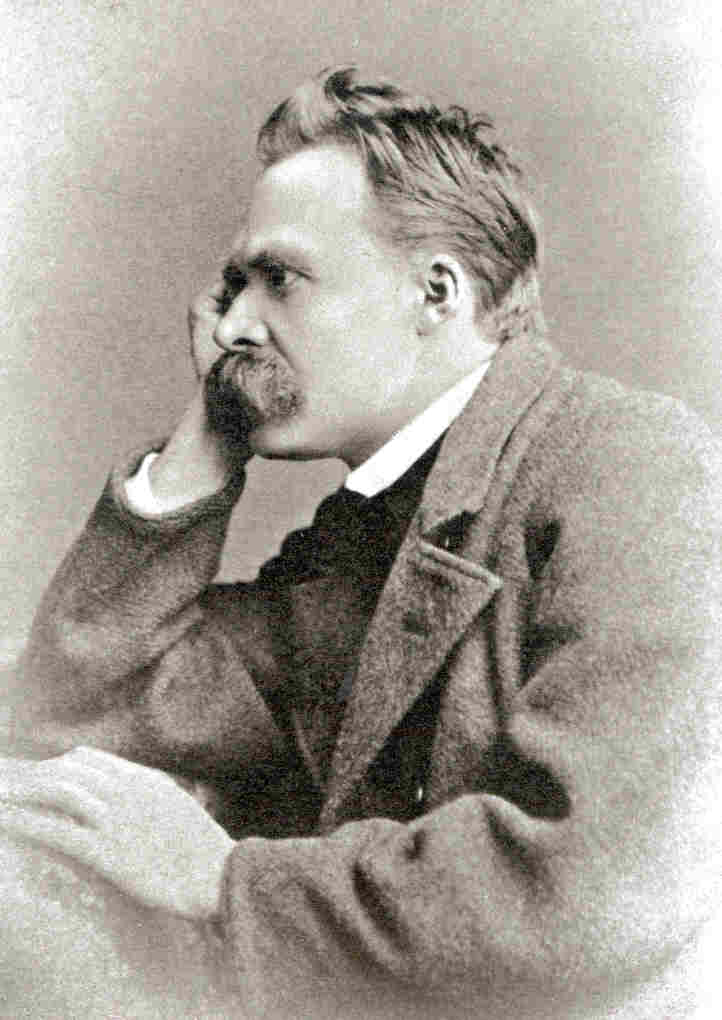
\includegraphics[height=4cm]{../../graphics/nietzsche.jpg}
            \end{column}
            \begin{column}{7cm}
                \begin{enumerate}
                    \item What is the value of (our) moral values?
                    \item What are the conditions and circumstances that give rise to these values?
                \end{enumerate}
            \end{column}
        \end{columns}
\end{frame}

We can begin to make sense of Nietzsche's question by reflecting on an important moral insight of Aristotle's. Aristotle believed that there was an important connection between conforming our actions to the dictates of morality and what he described as \emph{eudaemanaia}. Eudaemanaia is difficult to define, but we can understand it as meaning, roughly, human flourishing or living a life worth living. Aristotle's insight is that living a morally worthy life is, at the very least, a precondition of human flourishing. If we are to live a life worth living we must conform ourselves to the dictates of morality:
\begin{definition}\label{def:aristotle}
    The Aristotelian insight: Conforming our actions to the dictates of morality ought to promote human flourishing.
\end{definition}
If the Aristotelian insight is correct, then we can understand the \emph{value} of our moral values as consisting in the promotion of human flourishing. \change

\begin{frame}<presentation>[label=slide4]
    \frametitle{The Aristotelian Insight}
        \begin{columns}
            \begin{column}{3cm}
                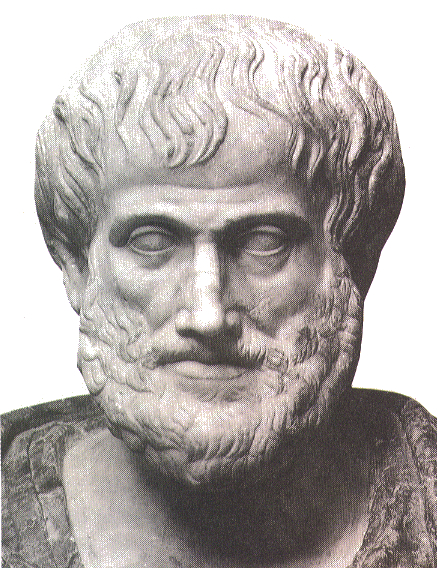
\includegraphics[height=4cm]{../../graphics/aristotle.jpg}
            \end{column}
            \begin{column}{7cm}
                \alert{The Aristotelian insight:} Conforming our actions to the dictates of morality ought to promote human flourishing.
            \end{column}
        \end{columns}
\end{frame}

So the first point that must be made if we are to make sense of the question at the heart of the \emph{Genealogy} is that the value of our values consist precisely in the degree to which they promote human flourishing or, as Nietzsche puts it, ``the growth of the plant `man'''. The second point that must be made, if we are to understand Nietzsche's question, is that Nietzsche denies that there is a single unifed phenomenon, morality, which it would make sense to be universally in favor or opposed to. Nietzsche denies that terms like ``morality'' refer everywhere and always to items with the same defining characteristics. There isn't any ``essence of morality'', that is, any set of defining properties that all and only instances of morality must exhibit. Nietzsche's view is rather like that which Wittgenstein was to develop fifty or sixty years hence: morality encompasses a wide variety of different things that are best connected one to another by ``family resemblances''. There is no essence of morality; rather there are difference constellations of practices, beliefs, and institutions that have very different origins, internal structures, motivations, and social functions. Each constellation, however, has sufficient similarity to some other constellation to allow the same word ``morality'' to be used of all of them. There is no single respect in which all moralities resemble one another. Rather they display a pattern of resemblance like that exhibited among members of a family. Family members are visually similar to one another but not in all in the same respect. The son may have his mother's eyes and his father's brow, a brow shared, perhaps, by the brother, whose own eyes are more akin to his father's, but whose chin more resemblance bears to the mother's. Yet despite there being no one set of common features common to all the members of the family, there is sufficient similarity in various different respects for them to be immediately recognized as being precisely that, a family. Similarly the different constellation of practices, beliefs, and so on sufficiently resemble one another in different respects for them to count as moralities. What counts as ``sufficient'' similarity is antecedently indeterminate---there are no antecedently specificable limits as to what counts as sufficient resemblance to make the term ``morality'' correctly applicable. Nietzsche sometimes puts this point by saying that there is no clear and sharp distinction between literal and metaphorical usage or between the proper or extended sense of a term.

There are indefinitely many different kinds of (possible and actual) things that could be called ``morality'' without impropriety. Despite the variability of what has been called ``morality'', in 19th century Europe ``morality'' had come to be used most commonly to designate one particular form of morality, important parts of which were ultimately derived from Christianity. Specifically, Christian morality had predominated in the recent past (until the beginning of the 19th century) and may have just recently (the middle of the 19th century) begun to be displaced by other forms of morality. Nevertheless, Christian morality was still dominant in the sense that it governed widespread areas of life, had a quasi-official standing and more importantly defined the terms in which people thought and spoke of morality.

Given Nietzsche's historical context and given his anti-essentialism, it is not odd for him to follow widespread usage and use ``morality'' to designate the specifically Christian (or immediately post-Christian) morality of 19th century middle class Central Europeans. In reading Nietzsche, it is thus very important to try to determine in each particular case whether he is using ``morality'' in the narrow sense to mean 19th century Christian morality or in a more general sense.

So there are a variety of different practices that each count as morality despite there sharing no unique set of defining characteristics. It is thus legitimate to ask the value of each of these particular moralities in the sense of asking whether and to what degree they promote human prosperity. If a particular morality were to promote human flourishing, it would be positively valuable to the degree to which it does so. If however, some morality were to systematically interfere with a life worth living, then it would lack any positive value and indeed be negatively valuable to the degree to which it interferes with human flourishing.

We are now in a position to make sense of the question that Nietzsche poses. Perhaps it makes no sense to ask whether the good itself is valuable, but it \emph{does} make sense to ask whether the good \emph{as conceived by 19th century Central Europeans} is valuable in the sense of promoting human flourishing. For after all, it is possible that 19th century Christian morality is badly misconceived with the disastrous result that we moderns have forestalled our happiness and well-being. It is not a foregone conclusion that engaging in some particular, historically conditioned morality will promote human flourishing. It is thus intelligible that it should be an open question whether our actual moral valuations are themselves valuable---whether the good as presently conceived promotes human flourishing. Nietzsche is not so much questioning the value of the good in itself; rather, he is questioning the value of the good as conceived by 19th Century Christian moral practice.

The project of the \emph{Genealogy} is thus explicitly critical in character. We must not assume the value of our values---this is something that must be determined by genealogical inquiry:
\begin{quote}
    One has taken the value of these ``values'' as given, as factual, as beyond all question; one has hitherto never doubted or hesitated in the slightest degree in supposing ``the good man'' to be of greater value than ``the evil man'', of greater value in the sense of furthering the advancement and prosperity of man in general (the future of man included). But what if the reverse were true? What if a symptom of regression were inherent in the ``good'', likewise a danger, a seduction, a poison, a narcotic, through which the present was possibly living at the expense of the future? Perhaps more comfortably, less dangerously, at the same time in a meaner style, more basely?---So that  precisely morality would be to blame if the highest power and splendor actually possible to the type man was never in fact obtained? So that precisely morality was the danger of all dangers?
\end{quote}
In critically evaluating our moral values one must leave it open at the outset whether or not and to what degree such values are themselves positively or negatively valuable. As a matter of fact, the conclusion of Nietzsche's inquiry is that despite the positive effects of the ascetic morality of Christianity, it is a positive hindrance to human prosperity and vitality, that it is a kind of nihilism or European Buddhism---a will to nothingness. In thus opposing nineteenth century Christian morality, Nietzsche sometimes describes himself as an \emph{immoralist}. While describing himself as an immoralist, this claim must be rightly understood. Nietzsche is not rejecting the claims of morality per se, only the claims of a historically conditioned, moral practice that he believes hinders human prosperity. He is an immoralist only from the perspective of a moral practice that he rejects as being fundamentally opposed to life. \change

\begin{frame}<presentation>[label=slide5]
    \frametitle{Family of Resemblance}
        \begin{columns}
            \begin{column}{3cm}
                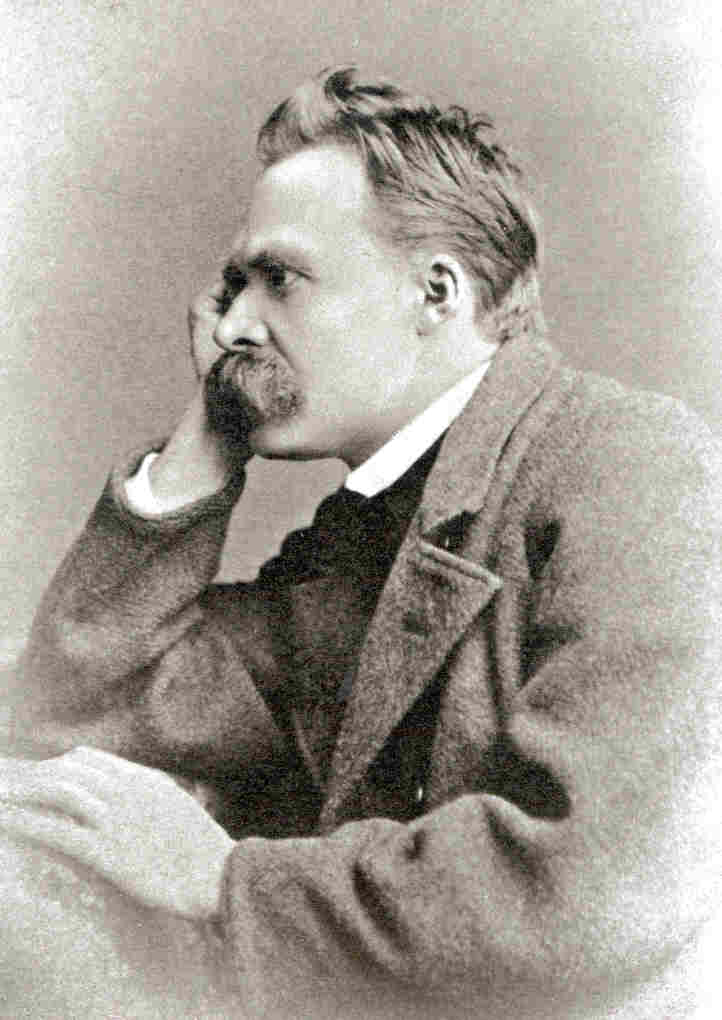
\includegraphics[height=4cm]{../../graphics/nietzsche.jpg}
            \end{column}
            \begin{column}{7cm}
                A concept \alert{C} is a family of resemblance concept if and only if there is no nontrivial feature \alert{F} that all and only things falling under \alert{C} share---rather things that fall under \alert{C} are sufficiently similar to one another in a number of different respects and there is no antecedently specifiable limit as to what counts as sufficient similarity.
            \end{column}
        \end{columns}
\end{frame}

While talk of a morality being positively or negatively valuable to the degree to which it helps or hinders human flourishing certainly helps in making sense of Nietzsche's questioning the value of our values, the metaphor of ``flourishing'' is perhaps to imprecise for us to attach a precise content of talk of ``the value of our values''. How valuable our morality is will, after all, depend on the degree to which it promotes human prosperity. And if we have no precise idea what human prosperity is, we will have no precise idea how valuable our morality is. It is also clear that different people in different historical circumstances have held a variety of different conceptions of the good life. So how are we to understand the operative metaphor of human flourishing?

Nietzsche has an idiosyncratic conception of human flourishing. Nietzsche identifies human flourishing with great concentrations and consciousness of what he calls the will to power. Nietzsche's conception of the will to power is easily misinterpreted and such misinterpretation is one of the sources of the view that he is a proto-Nazi and prophet of the Third Reich. So let's take some time to clarify in a preliminary fashion what he meant by ``will to power''. Both of the key concepts of this phrase, ``will'' and ``power'', are used by Nietzsche in a rather expansive sense.

Let's begin with the concept of will. Nietzsche's usage of ``will'' is rather elastic. He uses it to designate not only subpersonal drives and forces, but applies the concept as well to persons and institutions. An individual psychology will typically comprise a number of different drives or impulses not necessarily consistent with one another. Each of these Nietzsche designates as a will. Not only does Nietzsche speak of subpersonal forces as wills but he also speaks of the will of individuals. Thus, for example, he discusses at length Paul's priestly will being manifest in the moralizing interpretation he foists on the life of the historical Jesus. Not only are subpersonal forces and individuals designated as wills, but Nietzsche speaks as well of the will of institutions. Thus, for example, we can speak without impropriety of the will of the German nation, of UCL, and so on.

As to the concept of power, this too is used by Nietzsche in a rather expansive sense. Nietzsche's concept of power does not have a precise biological content. One might be tempted to interpret talk of the power of a species as designating the ability of a species to survive. This is not, however, how Nietzsche uses the term. Nietzsche explicitly acknowledges that one can sacrifice one's life in the interest of furthering one's will to power. Indeed, this is, Nietzsche maintains, the case with the historical Jesus. Jesus' acceptance of his crucifixion is interpreted as the highest manifestation of the will governing his radically non-moralizing way of life. Given that one can consistently sacrifice one's physical well-being to promote one's will to power, it is clear that talk of power has no biological content. Nor does it necessarily have political significance. While it is true that some individual's who Nietzsche praises as being the loci of high concentrations of the will to power have enjoyed great political power (notably Napoleon), others that Nietzsche praises have not. Thus Nietzsche claims that the author of \emph{Faust}, Goethe, displayed a remarkable degree and consciousness of the will to power. Goethe, however, had no political power to speak of in the Weimar Republic nor any political ambitions. So talk of power neither has a determinate biological or political content. What then did Nietzsche mean by it? One can only get a feel for Nietzsche's conception of the will to power by paying careful attention to the use to which he puts it. The historical exemplars of the will to power that Nietzsche explicitly mentions are a diverse lot, and the only thing they have in common is that they are in some sense worthy of our admiration. part of the problem in stating precisely what human flourishing consists is that Nietzsche denies that there is a unique way for individuals to flourish. Indeed, it is a mark or symptom of great strength of will that an individual will devise novel ways of living and novel values to accompany it. There is no one thing in which the good life consists but every way of flourishing will involve the manifestation of great strength of will.

To return to the question, a morality then is positively valuable to the extent to which it confers or helps to confer greater concentrations and consciousness of the will to power. It is the degree to which morality promotes human growth and vitality which is the standard by which it is critically evaluated. \change

\begin{frame}<presentation>[label=slide6]
    \frametitle{Will to Power}
        \begin{columns}
            \begin{column}{3cm}
                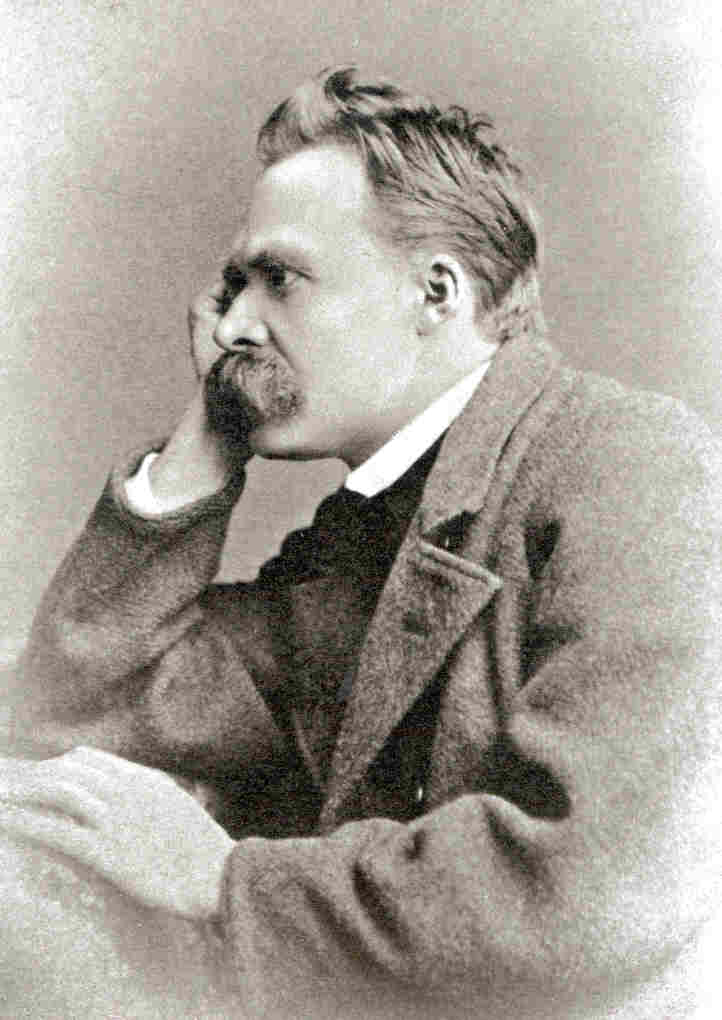
\includegraphics[height=4cm]{../../graphics/nietzsche.jpg}
            \end{column}
            \begin{column}{7cm}
                Human flourishing is high concentrations and consciousness of \alert{will to power}
            \end{column}
        \end{columns}
\end{frame}

How is a critique of values to be undertaken? What are the methods appropriate to it? How can we assess whether a particular morality promotes or hinders human prosperity? Nietzsche's insight, if it is one, is that in order to assess the value of morality we must have knowledge of the conditions and circumstances under which such moral valuations were devised:
\begin{quote}
    What are the conditions and circumstances under which our moral valuations were devised?
\end{quote}
Nietzsche maintains that in order to determine the value of our values we must first undertake the history of our moral practice.

There are a number of features of Nietzsche's historical approach that are worth emphasizing. First, undertaking a historiography of nineteenth century Christian morality is a means of achieving the requisite critical distance towards such moral valuations. If one were to conduct such an inquiry more or less a priori---``gazing around haphazardly in the blue'' as Nietzsche puts it---there is a danger in mistaking contingent, historically conditioned features of our morality with essential features of anything that deserves the name. Second without appealling to historical and philological evidence there is a danger of advancing questionable assumptions as historical truths. Thus according to Nietzsche:
\begin{quote}
    \ldots\ it must be obvious which color is a hundred times more vital for a genealogist of morals than blue: namely gray, that is, what is documented, what can actually be confirmed and has actually existed, in short the entire long hieroglyphic record, so hard to decipher, of the moral past of mankind!
\end{quote}
Third, there is an important constraint on an adequate inquiry into the origins of morality. Nietzsche resolutely insists that a history of morality be thoroughly naturalistic. As Hume emphasized, naturalism in philosophy can be understood in a variety of ways, but Nietzsche is a naturalist in one of the historically most important senses of the term. In this sense, naturalism is most fundamentally opposed to belief in the supernatural---deities, spirits, astral projections and the like. In determining the origins of moral practice, Nietzsche insists that we eschew any attributions of supernatural origin.

It is important to emphasize that genealogical inquiry is not a novel form of historiography. Some commentators, especially Michel Foucault, have spoke of Nietzsche's genealogical method as if it were a new method of historical inquiry. This is a mistake. Nietzsche explicitly speaks of genealogical predecessors, in particular, what he refers to as the ``English psychologists''. If by his own lights the English psychologists were undertaking a genealogical inquiry into the moral history of mankind then he cannot take himself to be instituting a novel form of historiography. Rather, As Alexander Nehemas has observed, genealogy just is history properly conducted.

Raymond Guess has usefully contrasted Nietzsche's genealogical method of inquiry with the practice of tracing a pedigree. This latter practice is at least as old as Western literature itself. Consider the following example of a pedigree from Book II of the \emph{Iliad}:
\begin{verse}
    Powerful Agamemnon \\
    Stood up holding the scepter Hephaistos \\
    Had wrought him carefully. \\
    Hephaistos gave it to Zeus the king, \\
    Son of Kronos \\
    And Zeus in turn gave it to the courier Argeiphontes, \\
    And lord Hermes gave it to Pelops, \\
    Driver of horses, \\
    And Pelops gave it to Atreus, the shepherd \\
    Of the people. \\
    Atreus dying left it to Thyestes \\
    Of the rich flocks \\
    And Thyestes left it in turn to Agamemnon \\
    To carry \\
    And to be lord over many islans \\
    And over all of Argos. \\
    Leaning upon this scepter he spoke \ldots \\
\end{verse}
This early example exhibits the main characteristics of what Guess calls a pedigree. The general point of tracing a pedigree of to legitimize or at the very least positively valorize some person, institution, of thing. In the present examole, that Agamemnon has inherited the ancestral scepter lends authority to his words and justifies his position as lord of Argos and the ``many islands''. The authority that the scepter provides Agamemnon is generally accepted by the other characters of the \emph{Iliad}. Even those critical of Agamemnon recognize the authority that the scepter endows him---thus Diomedes' bitter remark that although Zeus gave Agamemnon the scepter ``he did not give you a heart, and of all the power this is the greatest''.

Homer's pedigree of the scepter traces Agamemnon's possession of it back through a series of unbroken steps to a singular origin. For a pedigree to work, that is, for it to legitimize or positively valorize some item, the origin must be the source of the positive value, and each of the steps of the transmission must be value preserving if not value enhancing. In this particular example, it is important that the scepter can be traced back to Hephaistos and Zeus---the former guarantees the quality of the workmanship and the latter guarantees the associated claim of political authority. Moreover, in order for each step of the transmission of the scepter to be value preserving, such that the owner of the scepter is invested with the requisite authority, it must proceed by voluntary donation. Thus Achilleus would fail to gain Agamemnon's position of lord of Argos and the ``many islands'' simply by wresting the scepter from him.

This kind of pedigree, then, has five main characteristics:
\begin{enumerate}
    \item The function of a pedigree is to legitimize or positively valorize some item
    \item The pedigree begins from some singular origin
    \item The singular origin is the source of the value of that item
    \item The pedigree traces an unbroken line of transmission from the origin to the target item
    \item The steps of the transmission preserve or enhance the value in question
\end{enumerate}

Nietzsche's use of genealogy differs from tracing a pedigree in all five respects. Nietzsche certainly doesn't undertake a genealogy of nineteenth century Christian moral practice with the intent of legitimizing or positively valorizing it. Indeed providing such a genealogy is the basis of its criticism. So whatever the proper function of genealogy turns out to be, it clearly differs from the function of a pedigree. Thus Nietzsche's genealogy differs from the practice of tracing a pedigree on the very first point.

With respect to the second point, a genealogy won't characteristically discover a singular origin for the object under investigation. Thus, as Nietzsche argues, Christian morality does not originate with the activity of a single person (the historical Jesus) or group of people (the disciples). Indeed one of the main points of the \emph{Genealogy of Morals} is that Christian morality is the product of a number of diverse lines of development. It is the result of, for example, the \emph{ressentiment} of slaves directed at their masters, a psychological connection between having debts and suffering pain that gets established in commercial transactions, a need to turn one's aggression against oneself as the result of urbanization, the ambition of the priestly caste to exercise dominion over others, and so on. Thus Nietzsche's genealogical inquiry discovers, not a singular origin for Christian morality, but rather a number of distinct sources.

Furthermore, with respect to the third point, the further back a genealogical inquiry is pursued the less likely we shall discover something that we positively value. Thus Nietzsche claims that the origin of the concepts of ``guilt'', ``conscience'', and ``duty'' is ``like the beginnings of everything great on earth, soaked in blood thoroughly and for a long time''. Part of the point of this observation is to resist the sentimental assumption that things that we now value have origins that we would also value. Nietzsche believe that this assumption has distorted the results of traditional historiography and is itself a symptom of moral debility. The important point is that whatever value a thing now possesses the source of such value need not reside in its origin.

With respect to the fourth point, genealogical inquiry won't uncover a linearly ordered sequence of events that underlie the object of investigation. To see this, compare the graphic representations of the pedigree of Agamemnon's scepter with Nietzsche's genealogy of Christian morality. Whereas the pedigree of Agamemnon's scepter is linear, Nietzsche's genealogy of Christian morality has an elaborate branching structure.

Finally with respect to the fifth point, the historical events uncovered by genealogical inquiry do not preserve or transmit some antecedent value so much as they create or institute it. The decisive events that give rise to Christian morality, for example, do not transmit the values instituted at its origin; rather these events themselves institute such values. \change

\begin{frame}<presentation>[label=slide7]
    \frametitle{Guess on Pedigrees}
        \begin{columns}
            \begin{column}{3cm}
                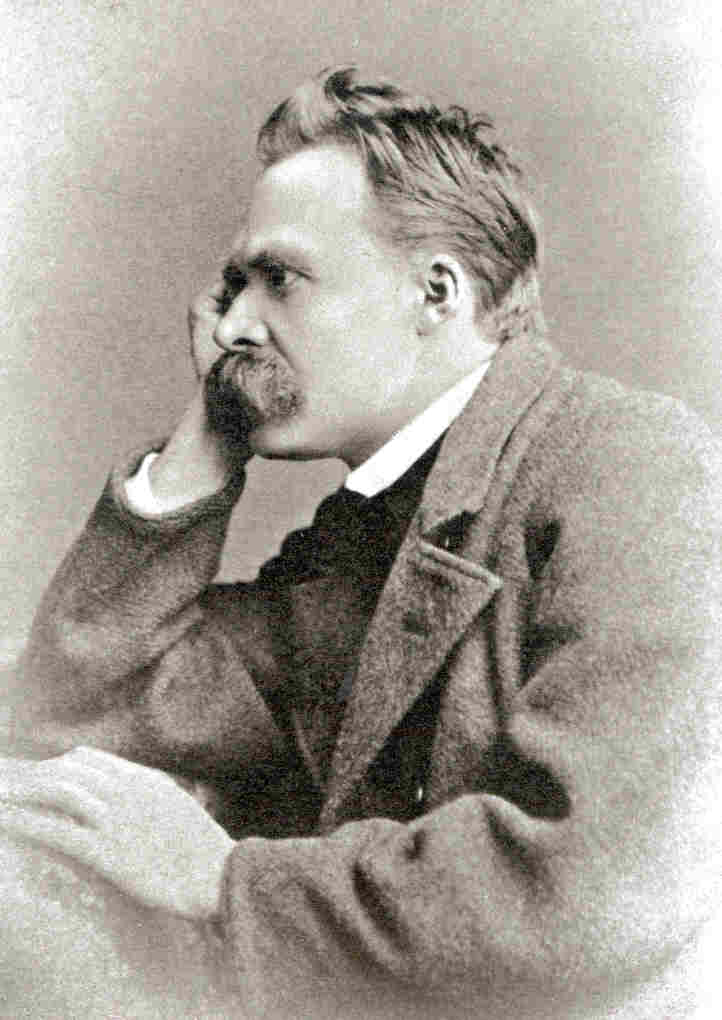
\includegraphics[height=4cm]{../../graphics/nietzsche.jpg}
            \end{column}
            \begin{column}{7cm}
                \begin{enumerate}
                    \item The function of a pedigree is to legitimize or positively valorize some item
                    \item The pedigree begins from some singular origin
                    \item The singular origin is the source of the value of that item
                    \item The pedigree traces an unbroken line of transmission from the origin to the target item
                    \item The steps of the transmission preserve or enhance the value in question
                \end{enumerate}
            \end{column}
        \end{columns}
\end{frame}

% section the_project_of_the_genealogy (end)

% \section*{Summary}

\end{document}
